% !TEX root = ../PolycopiePremiere2627.tex
%%%%%%%%%%%%%%%%%%%%%%%%%%%%%%%%%%%%%%%%%%%%%%%%%%%%%%%%%%%%%%%%%%%%%%%%%%%%%%%%
% Contenu initial repris de Louis Paternault --- http://ababsurdo.fr
%
% Publié sous licence Creative Commons Attribution-ShareAlike 4.0 International (CC BY-SA 4.0)
% http://creativecommons.org/licenses/by-sa/4.0/deed.fr
%%%%%%%%%%%%%%%%%%%%%%%%%%%%%%%%%%%%%%%%%%%%%%%%%%%%%%%%%%%%%%%%%%%%%%%%%%%%%%%%

\chapter{Informations chiffrées}

\section{Nuage de points et Point moyen}

\Dfn{Chaque point d'un \textcolor{J1}{nuage de points} représente un individu, dont les deux caractères étudiés correspondent aux coordonnées de ce point.}

\Dfn{Étant donné un ensemble de points $M_1(x_1;y_1)$, $M_2(x_2;y_2)$, …, $M_n(x_n;y_n)$, on définit le \textcolor{J1}{point moyen} comme le point, noté ici $G$, dont les coordonnées sont la moyenne arithmétique des coordonnées des points de l'ensemble :
\[
    G\left(\frac{x_1+x_2+\cdots+x_n}{n};\frac{y_1+y_2+\cdots+y_n}{n}\right)
\]}

\bigskip

\noindent\textbf{Activité}

Voici le poids à vide (approximatif) et la longueur des voitures les plus vendues en France\footnote{Sources : \emph{Auto moto} et \emph{www.fiches-auto.fr}, compilé par les contributeurs et contributrices de Wikipedia dans l'article \url{https://fr.wikipedia.org/wiki/Voitures_les_plus_vendues_en_France}} dans les années 1960 d'une part, et 2010 d'autre part.

\begin{center}
\begin{tabular}{|M{2.6cm}|M{3cm}|M{2.2cm}|M{2.2cm}|}
    \hline
    \textbf{Année} & \textbf{Modèle} & \textbf{Poids (kg)} & \textbf{Longueur (m)} \tabularnewline
    \hline
    1960 et 1961 & Renault Dauphine & 630 & 3,945 \tabularnewline
    \hline
    1962 à 1965 & Renault 4 & 540 & 3,609 \tabularnewline
    \hline
    1966 & Citroën Ami 6 & 800 & 3,960 \tabularnewline
    \hline
    1967 et 1968 & Renault 4 & 540 & 3,609 \tabularnewline
    \hline
    1969 & Peugeot 204 & 900 & 3,900 \tabularnewline
    \hline
    2010 & Peugeot 207 & 1250 & 4,030 \tabularnewline
    \hline
    2011 et 2012 & Renault Clio III & 1150 & 4,100 \tabularnewline
    \hline
    2013 à 2018 & Renault Clio IV & 1215 & 4,062 \tabularnewline
    \hline
    2019 & Peugeot 208 I & 1100 & 3,972 \tabularnewline
    \hline
\end{tabular}
\end{center}

\begin{enumerate}
    \item Représenter ces données sous la forme d'un nuage de points (dont les abscisses sont le poids, et les ordonnées la taille), en choisissant deux couleurs différentes pour les voitures des années 1960 et 2010.

        \begin{center}
            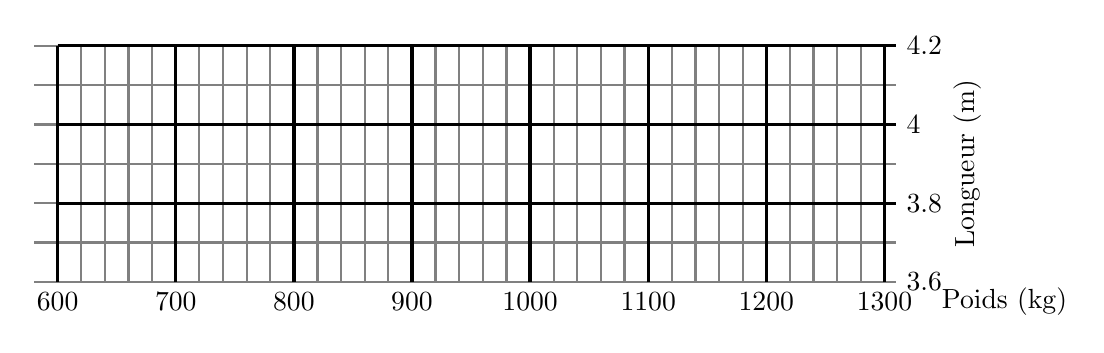
\begin{tikzpicture}[thick, xscale=1.5, yscale=5]
                \draw[gray] (5.8, 3.6) grid[xstep=.2, ystep=.1] (13.1, 4.2);
                \draw[very thick] (6, 3.6) grid[xstep=1, ystep=.2] (13.1, 4.2);
                \foreach \x in {6, 7, ..., 13} {
                    \draw (\x, 3.55) node {\x00};
                }
                \draw (13.4, 3.55) node[anchor=west] {Poids (kg)};
                \foreach \y in {3.6, 3.8, ..., 4.2} {
                    \draw (13.1, \y) node[right]{\y};
                }
                \draw (13.7, 3.9) node[rotate=90]{Longueur (m)};
            \end{tikzpicture}
        \end{center}
    \item Calculer les coordonnées du point moyen de chacune des deux séries, et les représenter sur le graphique.
    \item Commenter : Comment ont évolué le poids et la taille des voitures en cinquante ans ?
\end{enumerate}

\pagebreak

\section{Ajustement affine, Interpolation et Extrapolation}

\noindent\textbf{Activité}

Le nuage de points suivant présente la température mensuelle moyenne mesurée en décembre par une station météorologique aux environs de Lyon, de 1990 à 2025\footnote{Source : \emph{Messages climat — Mensuel}, par Météo France, \url{https://meteo.data.gouv.fr/datasets/6a183217f8648518b7101a3b}.}.

\begin{center}
    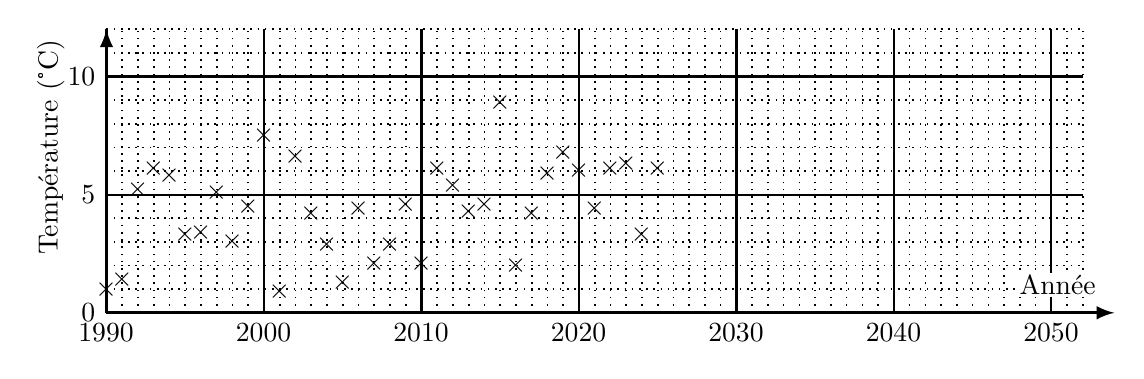
\begin{tikzpicture}[very thick, xscale=20, yscale=.3]
        % C'est très moche comme manière de faire pour tracer un graphique,
        % mais il est tard et je n'arrive pas à faire en sorte que pgfplots fasse ce que je veux.
        \foreach \annee in {1990, 2000, ..., 2050} {
            \draw ({\annee/100}, 0) node[below]{\annee};
            \draw[thick] ({\annee / 100}, 0) -- ++(0, 12);
        }
        \foreach \annee in {1990, 1991, ..., 2052} {
            \draw[semithick, dotted] ({\annee / 100}, 0) -- ++(0, 12);
        }
        \foreach \temperature in {0, 1, ..., 12} {
            \draw[semithick, dotted] (19.9, \temperature) -- (20.52, \temperature);
        }
        \foreach \temperature in {0, 5, ..., 12} {
            \draw (19.9, \temperature) node[left, anchor=east]{\temperature};
            \draw[thick] (19.9, \temperature) -- (20.52, \temperature);
        }
        \draw[-latex] (19.9, 0) -- (20.54, 0) node[above left=.5em, fill=white, inner sep=1pt]{Année};
        \draw[-latex] (19.9, 0) -- (19.9, 12) node[left=2em, rotate=90]{Température (\textdegree C)};
        \foreach \annee / \temperature in {
            1990 / 1,
            1991 / 1.4,
            1992 / 5.2,
            1993 / 6.1,
            1994 / 5.8,
            1995 / 3.3,
            1996 / 3.4,
            1997 / 5.1,
            1998 / 3,
            1999 / 4.5,
            2000 / 7.5,
            2001 / 0.9,
            2002 / 6.6,
            2003 / 4.2,
            2004 / 2.9,
            2005 / 1.3,
            2006 / 4.4,
            2007 / 2.1,
            2008 / 2.9,
            2009 / 4.6,
            2010 / 2.1,
            2011 / 6.1,
            2012 / 5.4,
            2013 / 4.3,
            2014 / 4.6,
            2015 / 8.9,
            2016 / 2,
            2017 / 4.2,
            2018 / 5.9,
            2019 / 6.8,
            2020 / 6,
            2021 / 4.4,
            2022 / 6.1,
            2023 / 6.3,
            2024 / 3.3,
            2025 / 6.1
        }{
            \draw ({\annee / 100}, \temperature) node{$\times$};
        }
    \end{tikzpicture}
\end{center}

Si la tendance se poursuit, quelle sera la température moyenne en décembre 2050 ?

\Dfn{Une \textcolor{J1}{droite d'ajustement} est une droite approchant au mieux un nuage de points.
Plusieurs méthodes existent pour déterminer une telle droite (droite de Mayer, moindres carrés), mais cette année, cette droite sera tracée au jugé.}

\Dfn{
\begin{itemize}
    \item \textcolor{J1}{Interpoler}, c'est déterminer une valeur manquante à l'intérieur d'une série de données.
    \item \textcolor{J1}{Extrapoler}, c'est déterminer une valeur manquante à l'extérieur d'une série de données.
\end{itemize}}

\Exemple{Reprenons le nuage de points de l'activité précédente (températures moyennes de décembre, de 1990 à 2025), et cherchons la température moyenne prévisible en 2050.

\medskip

\textbf{Etape 1} : on calcule les coordonnées du point moyen $G$ du nuage, qui sert de point d'appui pour tracer la droite d'ajustement au jugé.\\
\textcolor{J1}{L'abscisse moyenne des 36 années 1990 à 2025 est $\bar{x}=\dfrac{1990+2025}{2}=2007{,}5$, et la moyenne des 36 températures relevées est $\bar{y}\approx 4{,}4$. Donc $G(2007{,}5\ ;\ 4{,}4)$.}

\medskip

\textbf{Etape 2} : on trace, au jugé, la droite passant par $G$ et suivant au mieux l'allure générale du nuage, puis on la prolonge jusqu'à l'année 2050.\\
\textcolor{J1}{Comme 2050 n'appartient pas à l'intervalle $[1990\ ;\ 2025]$ des années observées, prolonger la droite jusqu'à cette valeur est bien une \emph{extrapolation}.}

\medskip

\textbf{Etape 3} : on lit, sur le graphique, l'ordonnée du point de la droite d'abscisse 2050.\\
\textcolor{J1}{On obtient une température moyenne prévisible d'environ 7\textdegree C en décembre 2050 --- un résultat approximatif, puisqu'il dépend de la droite tracée à main levée.}
}

\section{Tableau croisé d'effectifs}

\Dfn{Un \textcolor{J1}{tableau croisé d'effectifs} (ou table de contingence) présente les effectifs obtenus en croisant deux caractères observés sur une même population. Les totaux inscrits en marge de chaque ligne et de chaque colonne, appelés \textcolor{J1}{effectifs marginaux}, donnent, pour chaque modalité d'un des deux caractères, l'effectif total toutes modalités de l'autre caractère confondues.}

\bigskip

\Exemple{Dans un lycée, on interroge les élèves de première sur leur choix de suivre (ou non) l'enseignement de spécialité Mathématiques. Voici les effectifs obtenus, selon le sexe.

\begin{center}
\begin{tabular}{|l|c|c|c|}
    \hline
     & \textbf{Filles} & \textbf{Garçons} & \textbf{Total} \\
    \hline
    \textbf{Suivent la spécialité Maths} & 40 & 60 & \textcolor{J1}{100} \\
    \hline
    \textbf{Ne suivent pas la spécialité} & 80 & 40 & \textcolor{J1}{120} \\
    \hline
    \textbf{Total} & \textcolor{J1}{120} & \textcolor{J1}{100} & \textcolor{J1}{220} \\
    \hline
\end{tabular}
\end{center}

\medskip

\textbf{Etape 1} : on complète les effectifs marginaux en additionnant chaque ligne, puis chaque colonne (le total général s'obtient de deux façons --- en sommant les totaux de lignes, ou ceux des colonnes --- ce qui permet de vérifier le tableau).\\
\textcolor{J1}{Ligne « spécialité » : $40+60=100$. Ligne « pas de spécialité » : $80+40=120$. Colonne « Filles » : $40+80=120$. Colonne « Garçons » : $60+40=100$. Total général : $100+120=120+100=220$.}

\medskip

\textbf{Etape 2} : quelle proportion des élèves suivant la spécialité Mathématiques sont des filles ?\\
\textcolor{J1}{Parmi les 100 élèves qui suivent la spécialité, 40 sont des filles, soit une proportion de $\dfrac{40}{100}=0{,}4=40\,\%$.}
}

\section{Diagrammes}

\Prp{Dans un diagramme circulaire, les angles de chacune des sections sont \textcolor{J1}{proportionnels} aux effectifs correspondants.}

\Exemple{
    \begin{multicols}{2}
    Le tableau ci-contre représente le temps quotidien passé à réaliser des tâches ménagères, par les hommes et les femmes\footnote{Source : \emph{Femmes et hommes - Regards sur la parité}, \textsc{Insee}, 2012, \url{https://www.insee.fr/fr/statistiques/1372773?sommaire=1372781&q=taches+domestiques}}.

        \columnbreak

        \begin{center}
            \begin{tabular}{|r|c|c|c|}
                \hline
                & \textbf{1986} & \textbf{1999} & \textbf{2010} \\
                \hline
                Hommes & 2h07 & 2h13 & 2h13 \\
                \hline
                Femmes & 5h07 & 4h36 & 4h01 \\
                \hline
            \end{tabular}
        \end{center}
    \end{multicols}

    Représentons, sous la forme d'un diagramme circulaire, la répartition entre hommes et femmes du temps consacré aux tâches ménagères en 2010.

    \medskip

    \textbf{Etape 1} : on convertit les deux durées dans la même unité (les minutes), puis on calcule leur somme.\\
    \textcolor{J1}{Hommes : $2\text{h}13 = 133$ min. Femmes : $4\text{h}01=241$ min. Total : $133+241=374$ min.}

    \medskip

    \textbf{Etape 2} : d'après la propriété précédente, l'angle de chaque secteur est proportionnel à la durée qu'il représente ; on applique un produit en croix sur $360$\textdegree.\\
    \textcolor{J1}{Secteur « Hommes » : $\dfrac{133}{374}\times 360 \approx 128$\textdegree. Secteur « Femmes » : $\dfrac{241}{374}\times 360 \approx 232$\textdegree\ (on vérifie bien que $128+232=360$).}

    \medskip

    \textbf{Etape 3} : on reporte ces deux angles au rapporteur pour tracer le diagramme circulaire.

    \begin{center}
        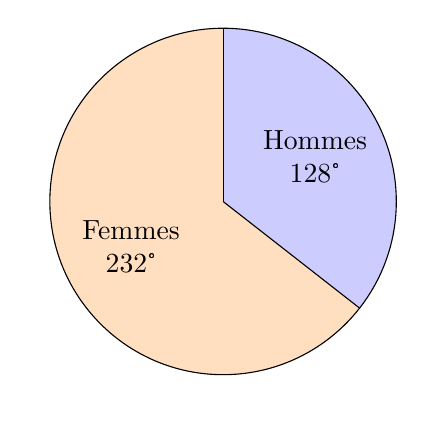
\begin{tikzpicture}
            \fill[blue!20] (0,0) -- (90:2.2) arc (90:-38:2.2) -- cycle;
            \fill[orange!25] (0,0) -- (-38:2.2) arc (-38:-270:2.2) -- cycle;
            \draw (0,0) circle (2.2);
            \draw (0,0) -- (90:2.2);
            \draw (0,0) -- (-38:2.2);
            \node[align=center] at (26:1.3) {Hommes\\128\textdegree};
            \node[align=center] at (206:1.3) {Femmes\\232\textdegree};
        \end{tikzpicture}
    \end{center}
}
